%% This is file `elsarticle-template-1-num.tex',
%%
%% Copyright 2009 Elsevier Ltd
%%
%% This file is part of the 'Elsarticle Bundle'.
%% ---------------------------------------------
%%
%% It may be distributed under the conditions of the LaTeX Project Public
%% License, either version 1.2 of this license or (at your option) any
%% later version.  The latest version of this license is in
%%    http://www.latex-project.org/lppl.txt
%% and version 1.2 or later is part of all distributions of LaTeX
%% version 1999/12/01 or later.
%%
%% The list of all files belonging to the 'Elsarticle Bundle' is
%% given in the file `manifest.txt'.
%%
%% Template article for Elsevier's document class `elsarticle'
%% with numbered style bibliographic references
%%
%% $Id: elsarticle-template-1-num.tex 149 2009-10-08 05:01:15Z rishi $
%% $URL: http://lenova.river-valley.com/svn/elsbst/trunk/elsarticle-template-1-num.tex $
%%
\documentclass[preprint,review,12pt]{elsarticle}

%% Use the option review to obtain double line spacing
%% \documentclass[preprint,review,12pt]{elsarticle}

%% Use the options 1p,twocolumn; 3p; 3p,twocolumn; 5p; or 5p,twocolumn
%% for a journal layout:
%% \documentclass[final,1p,times]{elsarticle}
%% \documentclass[final,1p,times,twocolumn]{elsarticle}
%% \documentclass[final,3p,times]{elsarticle}
%% \documentclass[final,3p,times,twocolumn]{elsarticle}
%% \documentclass[final,5p,times]{elsarticle}
%% \documentclass[final,5p,times,twocolumn]{elsarticle}

%% if you use PostScript figures in your article
%% use the graphics package for simple commands
\usepackage{graphics}
%% or use the graphicx package for more complicated commands
\usepackage{graphicx}
%% or use the epsfig package if you prefer to use the old commands
\usepackage{epsfig}
\usepackage{epstopdf}
%% The amssymb package provides various useful mathematical symbols
\usepackage{amssymb}
%% The amsthm package provides extended theorem environments
%% \usepackage{amsthm}

%% The lineno packages adds line numbers. Start line numbering with
%% \begin{linenumbers}, end it with \end{linenumbers}. Or switch it on
%% for the whole article with \linenumbers after \end{frontmatter}.
%% \usepackage{lineno}

%% natbib.sty is loaded by default. However, natbib options can be
%% provided with \biboptions{...} command. Following options are
%% valid:

%%   round  -  round parentheses are used (default)
%%   square -  square brackets are used   [option]
%%   curly  -  curly braces are used      {option}
%%   angle  -  angle brackets are used    <option>
%%   semicolon  -  multiple citations separated by semi-colon
%%   colon  - same as semicolon, an earlier confusion
%%   comma  -  separated by comma
%%   numbers-  selects numerical citations
%%   super  -  numerical citations as superscripts
%%   sort   -  sorts multiple citations according to order in ref. list
%%   sort&compress   -  like sort, but also compresses numerical citations
%%   compress - compresses without sorting
%%
%% \biboptions{comma,round}

% \biboptions{}
\usepackage{url}


\journal{Knowledge Based Systems}

\begin{document}

\begin{frontmatter}

%% Title, authors and addresses

%% use the tnoteref command within \title for footnotes
%% use the tnotetext command for the associated footnote;
%% use the fnref command within \author or \address for footnotes;
%% use the fntext command for the associated footnote;
%% use the corref command within \author for corresponding author footnotes;
%% use the cortext command for the associated footnote;
%% use the ead command for the email address,
%% and the form \ead[url] for the home page:
%%
%% \title{Title\tnoteref{label1}}
%% \tnotetext[label1]{}
%% \author{Name\corref{cor1}\fnref{label2}}
%% \ead{email address}
%% \ead[url]{home page}
%% \fntext[label2]{}
%% \cortext[cor1]{}
%% \address{Address\fnref{label3}}
%% \fntext[label3]{}

\title{A Graph Based Approach to Text Normalization}

%% use optional labels to link authors explicitly to addresses:
%% \author[label1,label2]{<author name>}
%% \address[label1]{<address>}
%% \address[label2]{<address>}

\author{}

\address{}

\begin{abstract}
%% Text of abstract

\end{abstract}

\begin{keyword}
%% keywords here, in the form: keyword \sep keyword
Text Normalization \sep Twitter \sep microblogs \sep social media
%% MSC codes here, in the form: \MSC code \sep code
%% or \MSC[2008] code \sep code (2000 is the default)

\end{keyword}

\end{frontmatter}

%%
%% Start line numbering here if you want
%%
% \linenumbers

%% main text

\section{Introduction}
\label{sec:introduction}

Social text has become an enormous part of our lives. We are moving towards to an era that we will be talking using machines more than we talk to each other. Social platforms make mass amounts of people communicate via typed or transcribed text. That is the era that the news are spreading digitally via social media other than edited newspaper articles.

This has been also starting of a new era for text analytics researches. The recent studies on social media such that Stock Prediction\cite{DBLP:conf/acl/SiMLLLD13}, politeness detection\cite{DBLP:conf/acl/Danescu-Niculescu-MizilSJLP13}, disaster detection\cite{Sakaki:2010:EST:1772690.1772777} tries to lighten up the road of this digitized future of ours.

Therefore analyzing social media text is a challenge for itself. Due to its noisy nature, many NLP tools are performing poorly on social media text\cite{ritter2010unsupervised}. The problems that noise in the social media text generates for NLP tools can be overcome by some preprocessing steps.

Unlike spoken and written language, digitized language has its own form and nature. Since the beginning of World Wide Web, internet has it's own slang. \textit{lol} meaning \textit{laughing out loudly},  \textit{xoxo} meaning \textit{kissing}, \textit{4u} meaning \textit{for you} are the oldest examples of this slang. Everyday new slangs as well as new words such as iTunes and new abbreviations are coming up. It is a huge, an evolving language that has long gone behind the reach and control of spellcheckers and slang dictionaries.
\begin{table}[tbhp]
\centering{}
\caption{Example of noisy tokens and their normalized form}
\label{tab:normalizations}
\begin{tabular}[h]{|r|r|}
\hline
ppl & people \\
havent & haven't \\
tmr &   tomorrow \\
soooo &  so \\
sooon &  soon \\
raight & right \\
raight & alright \\
r  &  are \\
\hline
\end{tabular}
\begin{tabular}[h]{|r|r|}
\hline
mor &    more \\
doin &   doing \\
n &      and \\
friiied &  fried \\
finge &  finger \\
kissin & kissing \\
u   &    you \\
\hline
\end{tabular}
\end{table}

Text normalization is a preprocessing step to restore noisy forms of text to its original(canonical) form\cite{Han:2011:LNS:2002472.2002520} to make use of NLP applications or more broadly to understand the digitized text better. For example \textit{talk 2 u later} can be normalized as \textit{talk to you later} or similarly \textit{enormoooos, enrmss, enourmos} cand be normalized as \textit{enormous}. Those noisy tokens are referred as Out of Vocabulary(OOV) words. Normalization task is restoring OOV words to their In Vocabulary(IV) form.

Not every OOV word should be normalized\cite{DBLP:conf/acl/HassanM13}.
However not every OOV word should be considered for normalization, an OOV word can given a vocabulary


In this paper we introduce a context aware graph based text normalization method that can normalize given noisy tokens in a social text.

\section{Method}
\label{sec:graph}

%Unsupervised and graph based context aware model:

%In our model we made use of both lexical, contextual and shallow properties of the noisy text which makes use of a weighted token co-occurrence graph.

In this paper, we propose a graph based approach that models both contextual similarity features and lexical similarity features among an OOV word to be a normalized and the candidate IV words. A high level overview of our system is shown in Figure~\ref{fig:overview}. An input text is first preprocessed by tokenizing and Part-Of-Speech (POS) tagging. If the text contains an OOV word, the normalization candidates are chosen by making use of the contextual features extracted from a pre-generated word-relatedness graph, as well as lexical similarity features based on edit distance, longest common subsequence ratio, and double metaphone distance. In addition, a slang dictionary is used as an external resource to enrich the normalization candidate set. The details of the approach is explained in the following sub-sections.

%%% FIGURE
\begin{figure}[htb]
\begin{center}
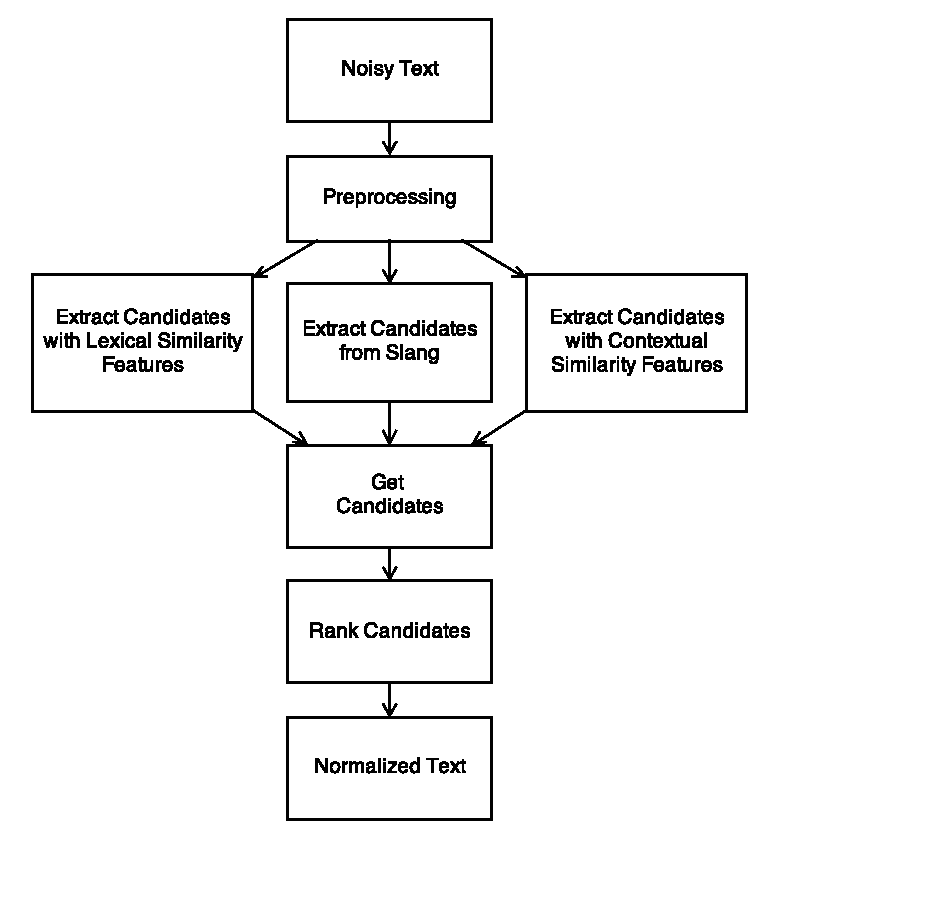
\includegraphics[scale=0.5]{overview}
\caption{High level overview of our system}
\label{fig:overview}
\end{center}
\end{figure}

\subsection{Preprocessing}

Tokenization is the first step in our system. Tokenization is the process of breaking the text into words, numbers, symbols, emoticons or in other words the smallest meaningful elements with the text called tokens. After tokenization we get POS tags of each token using a social media pos tagger. Unlike the normal pos taggers social media pos taggers~\cite{DBLP:conf/naacl/OwoputiODGSS13}\cite{Gimpel:2011:PTT:2002736.2002747} provides a broader set of tags that is special to social text. By this extended set of tags we can identify token such as discourse(rt for retweets, cont. for a tweet whose content follows up in the coming tweet) or urls and can process those tokens within their context.

As in Table~\ref{tab:postags}, after preprocessing each token is given a POS tag with a confidence measure. We later make use of this confidence scores calculating the weight of an edge in our context graph.

\begin{table}[htbp]
\begin{minipage}{.5\linewidth}
\begin{tabular}[h]{|llr|}
 \hline
Token & POS tag & Accuracy \\
 \hline
wit & P & 0.8793 \\
 \hline
a & D & 0.9959 \\
 \hline
beautiful & A & 0.9916 \\
 \hline
smil & G & 0.5311 \\
 \hline
\end{tabular}
\end{minipage}
\begin{minipage}{.5\linewidth}
\begin{tabular}[h]{|llr|}
 \hline
Token & POS tag & Accuracy \\
 \hline
w & P & 0.7486 \\
 \hline
a & D & 0.9920 \\
 \hline
beautiful & A & 0.9971 \\
 \hline
smile & N & 0.9712 \\
 \hline
\end{tabular}
\end{minipage}
\caption{POS tagger outputs of samples}
\label{tab:postags}
\end{table}


%% The Appendices part is started with the command \appendix;
%% appendix sections are then done as normal sections
%% \appendix

%% \section{}
%% \label{}

%% References
%%
%% Following citation commands can be used in the body text:
%% Usage of \cite is as follows:
%%   \cite{key}          ==>>  [#]
%%   \cite[chap. 2]{key} ==>>  [#, chap. 2]
%%   \citet{key}         ==>>  Author [#]

%% References with bibTeX database:
\bibliographystyle{model1-num-names}
\bibliography{sentic}

%% Authors are advised to submit their bibtex database files. They are
%% requested to list a bibtex style file in the manuscript if they do
%% not want to use model1-num-names.bst.

%% References without bibTeX database:

% \begin{thebibliography}{00}

%% \bibitem must have the following form:
%%   \bibitem{key}...
%%

% \bibitem{}

% \end{thebibliography}


\end{document}

%%
%% End of file `norm.tex'.
